%%
%% This is file `example.tex',
%% generated with the docstrip utility.
%%
%% The original source files were:
%%
%% coppe.dtx  (with options: `example')
%% 
%% This is a sample monograph which illustrates the use of `coppe' document
%% class and `coppe-unsrt' BibTeX style.
%% 
%% \CheckSum{1648}
%% \CharacterTable
%%  {Upper-case    \A\B\C\D\E\F\G\H\I\J\K\L\M\N\O\P\Q\R\S\T\U\V\W\X\Y\Z
%%   Lower-case    \a\b\c\d\e\f\g\h\i\j\k\l\m\n\o\p\q\r\s\t\u\v\w\x\y\z
%%   Digits        \0\1\2\3\4\5\6\7\8\9
%%   Exclamation   \!     Double quote  \"     Hash (number) \#
%%   Dollar        \$     Percent       \%     Ampersand     \&
%%   Acute accent  \'     Left paren    \(     Right paren   \)
%%   Asterisk      \*     Plus          \+     Comma         \,
%%   Minus         \-     Point         \.     Solidus       \/
%%   Colon         \:     Semicolon     \;     Less than     \<
%%   Equals        \=     Greater than  \>     Question mark \?
%%   Commercial at \@     Left bracket  \[     Backslash     \\
%%   Right bracket \]     Circumflex    \^     Underscore    \_
%%   Grave accent  \`     Left brace    \{     Vertical bar  \|
%%   Right brace   \}     Tilde         \~}
%%
\documentclass[dsc]{coppe}

\usepackage{booktabs}% tabelas mais bonitas
\usepackage{rotating}% rodando coisas, como tabelas
\usepackage{longtable} % tabelas longas
\usepackage[most]{tcolorbox} % caixas de texto
\usepackage{amsmath,amssymb}
\usepackage{hyperref}
\usepackage{listings} % para usar listagens

\makelosymbols
\makeloabbreviations

\begin{document}
  \title{Título da Tese}
  \foreigntitle{Thesis Title}
  \author{Nome do Autor}{Sobrenome}
  \advisor{Prof.}{Nome do Primeiro Orientador}{Sobrenome}{D.Sc.}
  \advisor{Prof.}{Nome do Segundo Orientador}{Sobrenome}{Ph.D.}
  \advisor{Prof.}{Nome do Terceiro Orientador}{Sobrenome}{D.Sc.}

  \examiner{Prof.}{Nome do Primeiro Examinador Sobrenome}{D.Sc.}
  \examiner{Prof.}{Nome do Segundo Examinador Sobrenome}{Ph.D.}
  \examiner{Prof.}{Nome do Terceiro Examinador Sobrenome}{D.Sc.}
  \examiner{Prof.}{Nome do Quarto Examinador Sobrenome}{Ph.D.}
  \examiner{Prof.}{Nome do Quinto Examinador Sobrenome}{Ph.D.}
  \department{PESC}
  \date{01}{2024}

  \keyword{Primeira palavra-chave}
  \keyword{Segunda palavra-chave}
  \keyword{Terceira palavra-chave}

  \maketitle

  \frontmatter
  \dedication{A alguém cujo valor é digno desta dedicatória.}

  \chapter*{Agradecimentos}

  Gostaria de agradecer a todos.

  \begin{abstract}

  Apresenta-se, nesta tese, ...

  \end{abstract}

  \begin{foreignabstract}

  In this work, we present ...

  \end{foreignabstract}

  \tableofcontents
  \listoffigures
  \listoftables
  \printlosymbols
  \printloabbreviations

  \mainmatter
  \chapter{Introdução}

  Este é um documento exemplo para o uso da classe CoppeTeX, destinado a ajudar os alunos da do Instituto Alberto Luiz Coimbra de Pós-graduação e Pesquisa de Engenharia (COPPE), da Universidade Federal do Rio de Janeiro.

  A classe \verb|coppe| foi criada por Vicente Helano e George Ainsworth, porém, em 2024, é mantida por Geraldo Xexéo e Eduardo Mangeli. Provavelmente Geraldo Xexéo, professor do Programa de Engenharia de Sistemas e Computação, deve continuar mantendo ou apoiando a manutenção por alguns anos. Se você quiser particiar do grupo de manutenção, é só entrar em contato.

  A versão mais atual dessa classe é mantida no GitHub, no repositório \url{https://github.com/COPPE-UFRJ/CoppeTeX}. De maneira arbitrária o prof. Geraldo Xexéo criou a organização COPPE-UFRJ no GitHub, e também está disposto a compartilhar com outras iniciativas semelhantes.

  Esse documento segue a norma de formatação de teses e dissertações da COPPE. Ele também pode ser usado para exames de qualificação. As principais instruções estão no documento que explica a classe, ``The \verb|coppe| document class'', que fica disponível no GitHub.

  Esse documento é usado como exemplo de coisas que podem ser feitas. Ele está configurado para usar citações do tipo author-data. Para usar citações do tipo numérica é necessário colocar, entre as opções de \verb|documentclass|, a opção \verb|numbers|.

  É importante de notar que essa classe não foi construída sobre a classe \LaTeX \  para a ABNT, e que segue de forma geral as regras da ABNT, mas não necessariamente de forma exata, já que o foco foi seguir as regras da Coppe. Essas mesmas regras da Coppe não especificam tudo que realmente seria necessário, então algumas coisas são decisões arbitrárias.

  Apesar desse modelo ser muito bom, ele tem um defeito: a limitação do sistema de referências criados. Primeiramente ele foi criado para o Bib\TeX, e não para o mais poderoso Bib\LaTeX, em segundo lugar, não foi criado de forma independente de linguagem, mas sim apenas para o Português, porque era a regra da época que as monografias deveriam ser exclusivamente em Português. Finalmente, o número de tipos de entrada é pequeno. Isso ainda não foi resolvido, mas está na fila para ser resolvido.

  Mais ainda, as regras da COPPE ainda não se adaptaram, no início de 2024, as novas regras da ABNT para citação, que são mais elegantes por não exigir o uso indiscriminado de maiúsculas.

  Este documento não substitui, mas complementa, o documento que descreve a classe.

\chapter{Configurações Iniciais}

   A primeira coisa a fazer é escolher o tipo de documento. Isso é feito como uma opção no comando inicial do arquivo, \verb|documentclass|. A classe \verb|coppe| suporta quatro formatos: tese de doutorado (\verb|dsc|), dissertação de mestrado (\verb|msc|), exame de qualificação de doutorado (\verb|dscexam|) e exame de qualificação de mestrado (\verb|mscexam|). Na verdade, o padrão da Coppe não cobre os exames de qualificação, mas é interessante seguir o padrão nesses casos também.

   Como pode ser visto nesse documento, muita coisa pode ser configurada, o que gerará o tratamento correto segundo as normas da COPPE. Para isso, logo após o \verb|\begin{document}| várias variáveis devem receber valor. Isso é feito com os comandos descritos que aparecem nesse exemplo.

   Recomendo ler o documento ``The \verb*|coppe| document class'' para entender melhor todas as opções disponíveis.

\section{Linguagem principal do texto}

  Essa classe considera que o texto principal está em português e algumas partes específicas, como o \textit{abstract}, estão em inglês. Caso o texto principal seja em inglês as seguintes opções devem ser usadas:
 \begin{itemize}
 \item A opção \verb|english| deve ser usada no comando \verb|\documentclass|.
 \item Os estilos de bibliografia usados devem ser \verb|en-coppe-plain.bst| ou \verb|en-coppe-unsrt.bst|
 \end{itemize}

  A variação de linguagem, em inglês ou português apenas, já é suportada pela classe Coppe\TeX  com o pacote Babel. Não é necessário incluí-lo.

\section{Por que usar o \LaTeX}

  Há uma grande discussão entre usuário de Word e \LaTeX, principalmente, quanto ao uso desses sistemas. Não é importante. Consideramos que ambos tem vantagens e desvantagens, e analisamos algumas em uma palestra introdutória que pode ser encontrada na rede.

  Nós escolhemos o \LaTeX por alguns motivos: grande facilidade de seguir um estilo sem se preocupar como, capacidade de gerenciar versões com software como git e sites como GitHub, funcionar em qualquer sistema operacional e  ser gratuito. Mais recentemente, o aparecimento de ferramentas de uso na rede permitiu o trabalho cooperativo muito facilitado.

  As principais desvantagens são: idiossincrasias que podem gastar tempo, pouco controle sobre algumas coisas sem se embrenhar nos detalhes da linguagem e ausência de um verdadeiro WYSIWYG \footnote{What you see is what you get, lembramos que o princípio do \LaTeX criticava esse conceito chamando de What you see is all you got}.

\section{Como e onde usar o \LaTeX}

  Existem muitos tutoriais de \LaTeX, mas basicamente, em 2024, ele é usado em dois ambientes:
  \begin{enumerate}
  \item Na sua máquina, instalando uma versão completa como o Mik\TeX, típico do Windows, ou simplesmente os pacotes padrão do Linux\footnote{Também existem versões para Mac, das quais eu não estou informado}.
  \item Usar um ambiente na rede, como o Overleaf.
  \end{enumerate}

  Em todo caso, recomendo fortemente que, ao mesmo tempo, mantenha versões no Git e faça o backup em sites como GitHub e GitLab. Isso pode ser feito em ambos os casos. Eu uso o GitHub sincronizado no Overleaf e na minha máquina com o GitHub Desktop. Muitas vezes troco quase que de forma transparente de um ambiente local para o da web sem nenhum problema.

\chapter{Algumas Regras da COPPE}

  Todas abreviaturas e símbolos devem ser definida antes de utilizada. Isso é facilmente feito usando os comandos para isso dedicados, tanto ativando a construção das listas de símbolos e abreviatura, como especificamente as declarando. Porém, muitos alunos não conseguem gerar a lista porque não sabem que é necessário rodar o comando \verb*|makeindex| de uma forma específica. Tudo está descrito no manual, porém é importante notar que isso pode ser feito automaticamente, inclusive no \textit{Overleaf}, usando o arquivo \verb*|latexmkrc|. Esse arquivo é pouco usado pelos usuários de \LaTeX, mas muito útil, e pode ser usado diretamente no Overleaf, ou rodando o comando \verb|latexmk| em uma linha de comando, ou mesmo rodando direto do menu no \TeX Studio.

  É imprescindível definir os símbolos, tal como o
  conjunto dos números reais $\mathbb{R}$ e o conjunto vazio $\emptyset$.
  \symbl{$\mathbb{R}$}{Conjunto dos números reais}
  \symbl{$\emptyset$}{Conjunto vazio}. Usamos esse exemplo aqui justamente para mostrar como devem ser usados os símbolos de Reais ($\mathbb{R}$), Inteiros ($\mathbb{Z}$), Complexos($\mathbb{C}$), Racionais (($\mathbb{Q}$)) Booleanos (($\mathbb{B}$)), etc.

  Para as listas de abreviaturas e símbolos funcionarem no Overleaf é necessário rodar o \verb|latexmkrc|. O Overleaf faz isso automaticamente. Caso haja um problema, verifique se o arquivo \verb|coppe.ist| está no diretório. Também é útil compilar do início e também apagar todos os arquivos desnecessários.

  Como as listas de símbolos e de abreviaturas usamo o mesmo comando usado para criar índices, e também não há uma expectativa que a tese tenha um índice, se for desejado criar índices é necessário tanto criar, ou adotar, um novo arquivo \verb*|.ist|, que define o formato do índice, como alterar o \verb*|latexmkrc| para fazer também esse passo. Ou fazer o passo de rodar o \verb*|makeindex| na mão.

\section{Citações}

 Citações curtas podem ser feitas \quote{o comando quote} ou direto com ``duas crases e dois apóstrofos.'' Citações longas devem usar o comando \verb*|longuote|

  \begin{longquote}
  Um exemplo de citação longa nas regras da ABNT (4cm de recuo e fonte menor)
  feita com o ambiente  \verb=longquote= The primary objective of this
  investigation was to determine the feasibility of detecting corrosion in
  aluminum Naval aircraft components with neutron radiographic interrogation
  and the use of standard corrosion penetrameters. Secondary objectives
  included the determination of the effect of object thickness on image quality,
  the defining of minimum levels of detectability and a preliminary investigation
  of a means whereby the degree of corrosion could be quantified with neutron
  radiographic data. \cite{article-example}
  \end{longquote}

  Citações devem apontar as referências. Para isso, está disponível o ótimo pacote \verb*|natbib| que permite criar citações em dois formatos, o totalmente dentro de parênteses (\verb*|\citep|), como em \citep{article-example} como o de citação pertencente ao texto, como em \citet{article-example}. Veja o capítulo sobre referências bibliográficas.

  Em todo caso, \textbf{deve se tomar enorme atenção com as citações, para evitar ocorrer em plágio não intencional}.

\chapter{Floats}

Grande parte dos problemas de iniciantes, e veteranos, em \LaTeX é da localização dos \textit{floats}, como figuras e tabelas. Para o bom comportamente é importante que sempre que usar um comando do tipo \verb*|\begin{figure}[hbt]| não sejam esquecidas as opções de posicionamento.

A regra geral de posicionamento é que uma figura ou quadro só pode aparecer a partir da mesma página onde é citado pela primeira vez, nunca antes. Normalmente eu sigo a ordem de preferência aqui, fim da página, topo da página, isto é \verb*|hbt|. Se desejado, pode ser usado o \verb*|p|, que coloca os floats em uma página única. Para forçar mais o posicionamento, é possível usar o pacote \verb*|float| e usar a opção \verb*|H|. Além disso é possível usar o pacote \verb*|placeins| que permite tanto definir que \textit{floats} devem sempre ser colocados na mesma seção ou outra regra, quanto usar o comando \verb*|FlaotBarrier|, que obriga a todos os \textit{floats} aparecerem.

\textbf{Segundo a norma da ABNT, as legendas} \verb|\caption| \textbf{das figuras e quadros ficam em baixo deles, enquanto as legendas das tabelas ficam em cima. }

Quadros são opcionais. Quando usados, tabelas passam a só conter números, enquanto quadros contém números e outras coisas. \textbf{O CoppeTeX ainda não suporta quadros!}

\section{Tabelas e Figuras Padrão}

Vamos ver uma tabela padrão, como a \autoref{tab:exemplo_numeros}.

\begin{table}[ht]
\centering % Centraliza a tabela
\caption{Exemplo de Tabela de Números}
\label{tab:exemplo_numeros}
\begin{tabular}{ccc} % Define a quantidade de colunas
\hline % Linha superior
\textbf{Coluna 1} & \textbf{Coluna 2} & \textbf{Coluna 3} \\ % Cabeçalhos
\hline % Linha média
1 & 2 & 3 \\ % Primeira linha de dados
\hline
4 & 5 & 6 \\ % Segunda linha de dados
\hline
7 & 8 & 9 \\ % Terceira linha de dados
\hline
10 & 11 & 12 \\ % Quarta linha de dados
\hline % Linha inferior
\end{tabular}
\end{table}

Já a \autoref{fig:exemplo_figura} é uma figura padrão, com controle da largura.

\begin{figure}[ht]
\centering % Centraliza a figura

\includegraphics[width=0.5\textwidth]{coppe-logo.pdf} % Inclui a imagem com metade da largura do texto
\caption{Exemplo de Figura com Legenda Abaixo} % Legenda da figura
\label{fig:exemplo_figura} % Etiqueta para referência cruzada
\end{figure}

\section{Tabelas mais elegantes}

Atualmente a tendência é usar tabelas mais leves, como \autoref{tab:exemplo_numerosbom}. Isso exige o pacote \verb*|booktabs|.

\begin{table}[ht]
\centering % Centraliza a tabela
\caption{Exemplo de Tabela de Números mais elegantes}
\label{tab:exemplo_numerosbom}
\begin{tabular}{ccc} % Define a quantidade de colunas
\toprule % Linha superior
\textbf{Coluna 1} & \textbf{Coluna 2} & \textbf{Coluna 3} \\ % Cabeçalhos
\midrule % Linha média
1 & 2 & 3 \\ % Primeira linha de dados
4 & 5 & 6 \\ % Segunda linha de dados
7 & 8 & 9 \\ % Terceira linha de dados
10 & 11 & 12 \\ % Quarta linha de dados
\bottomrule % Linha inferior
\end{tabular}
\end{table}

\section{Tabelas Longas ou Largas}

Se sua tabela é muito longa ou larga, existem várias opções.
\begin{itemize}
    \item alterar o tamanho da letra
    \item Usar o longtable
    \item rodar a tabela, fazendo ela em \textit{landscape}
    \item fazer a tabela dentro de um minibox
\end{itemize}

\subsection{Tabelas largas demais}

É comum em teses que as tabelas sejam largas demais. Há várias formas de resolver isso.

A \autoref{tab:tabela_largafns} é larga demais, e nela isso é resolvido diminuindo a fonte para \verb|\footnotesize|.

\begin{table}[ht]
\centering % Centraliza a tabela
\caption{Exemplo de Tabela Larga com Fonte Menor}
\label{tab:tabela_largafns}
\footnotesize % Aplica uma fonte menor para a tabela
\begin{tabular}{cccccccc} % Aumente o número de colunas conforme necessário
\toprule
\textbf{Coluna 1} & \textbf{Coluna 2} & \textbf{Coluna 3} & \textbf{Coluna 4} & \textbf{Coluna 5} & \textbf{Coluna 6} & \textbf{Coluna 7} & \textbf{Coluna 8} \\
\midrule
Dado 1.1 & Dado 1.2 & Dado 1.3 & Dado 1.4 & Dado 1.5 & Dado 1.6 & Dado 1.7 & Dado 1.8 \\
Dado 2.1 & Dado 2.2 & Dado 2.3 & Dado 2.4 & Dado 2.5 & Dado 2.6 & Dado 2.7 & Dado 2.8 \\
Dado 3.1 & Dado 3.2 & Dado 3.3 & Dado 3.4 & Dado 3.5 & Dado 3.6 & Dado 3.7 & Dado 3.8 \\
\bottomrule
\end{tabular}
\end{table}

O comando \verb|\resizebox{width}{height}{content}| permite ajustar o tamanho de qualquer coisa, inclusive uma tabela, como na \autoref{tab:examplerb}. No caso, estou fazendo a tabela ficar maior, para ocupar o espaço, mas funciona para qualquer tamanho.

\begin{table}[ht]
\centering
\caption{Exemplo de Tabela Redimensionada}
\label{tab:examplerb}
\resizebox{\textwidth}{!}{%
\begin{tabular}{llll}
\toprule
Coluna 1 & Coluna 2 & Coluna 3 & Coluna 4 \\
\midrule
Dados 1 & Dados 2 & Dados 3 & Dados 4 \\
Dados 5 & Dados 6 & Dados 7 & Dados 8 \\
\bottomrule
\end{tabular}%
}
\end{table}

Para rodar uma tabela muito larga em 90 graus no LaTeX, você pode usar o pacote \verb*|rotating|. Este pacote fornece o ambiente \verb*|sidewaystable|, que automaticamente gira a tabela, incluindo sua legenda, em 90 graus. Isso é especialmente útil para acomodar tabelas largas em documentos, garantindo que elas caibam na página sem comprometer a legibilidade.

Aqui está um exemplo de como usar o ambiente \verb*|sidewaystable| para girar uma tabela. Primeiro, apresento o código dentro de um ambiente verbatim para mostrar como ele deve ser escrito no seu documento \LaTeX. Em seguida, forneço o mesmo código fora do ambiente verbatim para demonstrar como ele funcionaria na prática. A tabela aqui é pequena, só para ilustrar.

\begin{sidewaystable}
\centering
\caption{Sua Legenda Aqui}
\label{tab:sua_tabela}
\begin{tabular}{lll}
\toprule
Coluna 1 & Coluna 2 & Coluna 3 \\
\midrule
Item 1 & Item 2 & Item 3 \\
Item 4 & Item 5 & Item 6 \\
\bottomrule
\end{tabular}
\end{sidewaystable}

Se a tabela for muito longa, o ambiente \verb|longtable| é o ideal. Ele fornece comandos para \textit{headers}, cabeçalhos, e \textit{footers} tanto no ínicio e no fim da tabela, como em todas as páginas. A \autoref{tab:longa} fornece um exemplo de 3 páginas.

\begin{longtable}{|c|c|c|}
\caption{Exemplo de Tabela Longa}\label{tab:longa} \\
\hline \textbf{Coluna 1} & \textbf{Coluna 2} & \textbf{Coluna 3} \\ \hline
\endfirsthead
\multicolumn{3}{c}%
{{\tablename\ \thetable{} -- continuação da página anterior}} \\
\hline \textbf{Coluna 1} & \textbf{Coluna 2} & \textbf{Coluna 3} \\ \hline
\endhead
\hline \multicolumn{3}{|r|}{{Continua na próxima página}} \\ \hline
\endfoot
\hline
\multicolumn{3}{|r|}{{Continua na próxima página}}\\
\hline \hline
\endlastfoot

1 & 2 & 3 \\
4 & 5 & 6 \\
1 & 2 & 3 \\
4 & 5 & 6 \\
1 & 2 & 3 \\
4 & 5 & 6 \\
1 & 2 & 3 \\
4 & 5 & 6 \\
1 & 2 & 3 \\
4 & 5 & 6 \\
1 & 2 & 3 \\
4 & 5 & 6 \\
1 & 2 & 3 \\
4 & 5 & 6 \\
1 & 2 & 3 \\
4 & 5 & 6 \\
1 & 2 & 3 \\
1 & 2 & 3 \\
4 & 5 & 6 \\
1 & 2 & 3 \\
4 & 5 & 6 \\
1 & 2 & 3 \\
4 & 5 & 6 \\
1 & 2 & 3 \\
4 & 5 & 6 \\
1 & 2 & 3 \\
4 & 5 & 6 \\
1 & 2 & 3 \\
4 & 5 & 6 \\
1 & 2 & 3 \\
4 & 5 & 6 \\
1 & 2 & 3 \\
4 & 5 & 6 \\
1 & 2 & 3 \\
4 & 5 & 6 \\
1 & 2 & 3 \\
4 & 5 & 6 \\
1 & 2 & 3 \\
4 & 5 & 6 \\
1 & 2 & 3 \\
4 & 5 & 6 \\1 & 2 & 3 \\
4 & 5 & 6 \\
1 & 2 & 3 \\
4 & 5 & 6 \\
1 & 2 & 3 \\
1 & 2 & 3 \\
4 & 5 & 6 \\
1 & 2 & 3 \\
4 & 5 & 6 \\
1 & 2 & 3 \\
4 & 5 & 6 \\
1 & 2 & 3 \\
4 & 5 & 6 \\
1 & 2 & 3 \\
4 & 5 & 6 \\
1 & 2 & 3 \\
4 & 5 & 6 \\
1 & 2 & 3 \\
4 & 5 & 6 \\
1 & 2 & 3 \\
4 & 5 & 6 \\
1 & 2 & 3 \\
4 & 5 & 6 \\
1 & 2 & 3 \\
4 & 5 & 6 \\
1 & 2 & 3 \\
4 & 5 & 6 \\
1 & 2 & 3 \\
4 & 5 & 6 \\
1 & 2 & 3 \\
4 & 5 & 6 \\
1 & 2 & 3 \\
4 & 5 & 6 \\
1 & 2 & 3 \\
4 & 5 & 6 \\
1 & 2 & 3 \\
4 & 5 & 6 \\
1 & 2 & 3 \\
4 & 5 & 6 \\
1 & 2 & 3 \\
4 & 5 & 6 \\
1 & 2 & 3 \\
4 & 5 & 6 \\
1 & 2 & 3 \\
4 & 5 & 6 \\
1 & 2 & 3 \\
4 & 5 & 6 \\
1 & 2 & 3 \\
4 & 5 & 6 \\
1 & 2 & 3 \\
4 & 5 & 6 \\
1 & 2 & 3 \\
4 & 5 & 6 \\
1 & 2 & 3 \\
4 & 5 & 6 \\
1 & 2 & 3 \\
4 & 5 & 6 \\
1 & 2 & 3 \\
4 & 5 & 6 \\
1 & 2 & 3 \\
4 & 5 & 6 \\
1 & 2 & 3 \\
4 & 5 & 6 \\
1 & 2 & 3 \\
4 & 5 & 6 \\
1 & 2 & 3 \\
4 & 5 & 6 \\

\end{longtable}

  \chapter{Revis\~ao Bibliogr\'afica}

  Para ilustrar a completa ades\~ao ao estilo de cita{\c c}\~oes e listagem de
  refer\^encias bibliogr\'aficas, a Tabela~\ref{tab:citation} apresenta cita{\c
  c}\~oes de alguns dos trabalhos contidos na norma fornecida pela CPGP da
  COPPE, utilizando o estilo numérico. Tirando do comando inicial o parâmetro opcional numérico, ele usará o nome-ano.

  \begin{table}[h]
  \caption{Exemplos de cita{\c c}\~oes utilizando o comando padr\~ao
    \texttt{\textbackslash cite} do \LaTeX\ e
    o comando \texttt{\textbackslash citet},
    fornecido pelo pacote \texttt{natbib}.}
  \label{tab:citation}
  \centering
  {\footnotesize
  \begin{tabular}{|c|c|c|}
    \hline
    Tipo da Publicação & \verb|\cite| & \verb|\citet|\\
    \hline
    Livro & \cite{book-example} & \citet{book-example}\\
    Artigo & \cite{article-example} & \citet{article-example}\\
    Relatório & \cite{techreport-example} & \citet{techreport-example}\\
    Relatório & \cite{techreport-exampleIn} & \citet{techreport-exampleIn}\\
    Anais de Congresso & \cite{inproceedings-example} &
      \citet{inproceedings-example}\\
    Séries & \cite{incollection-example} & \citet{incollection-example}\\
    Em Livro & \cite{inbook-example} & \citet{inbook-example}\\
    Dissertação de mestrado & \cite{mastersthesis-example} &
      \citet{mastersthesis-example}\\
    Tese de doutorado & \cite{phdthesis-example} & \citet{phdthesis-example}\\
    \hline
  \end{tabular}}
  \end{table}

 \begin{table}[h]
  \caption{Exemplos de cita{\c c}\~oes utilizando o comando padr\~ao
    \texttt{\textbackslash cite} do \LaTeX\ e
    o comando \texttt{\textbackslash citet},
    fornecido pelo pacote \texttt{natbib}. Além disso, usando o booktabs.}
  \label{tab:citation1}
  \centering
  {\footnotesize
  \begin{tabular}{ccc}
    \toprule
    Tipo da Publicação & \verb|\cite| & \verb|\citet|\\
    \midrule
    Livro & \cite{book-example} & \citet{book-example}\\
    Artigo & \cite{article-example} & \citet{article-example}\\
    Relatório & \cite{techreport-example} & \citet{techreport-example}\\
    Relatório & \cite{techreport-exampleIn} & \citet{techreport-exampleIn}\\
    Anais de Congresso & \cite{inproceedings-example} &
      \citet{inproceedings-example}\\
    Séries & \cite{incollection-example} & \citet{incollection-example}\\
    Em Livro & \cite{inbook-example} & \citet{inbook-example}\\
    Dissertação de mestrado & \cite{mastersthesis-example} &
      \citet{mastersthesis-example}\\
    Tese de doutorado & \cite{phdthesis-example} & \citet{phdthesis-example}\\
    \bottomrule
  \end{tabular}}
  \end{table}

\chapter{Alguns outros exemplo úteis}

\begin{tcolorbox}[title=Meu Textbox]
Este é o conteúdo do meu textbox. Você pode adicionar qualquer texto aqui, bem como incluir fórmulas matemáticas, listas e outros elementos que desejar. A caixa ajustará automaticamente o tamanho para acomodar seu conteúdo.
\end{tcolorbox}

\begin{tcolorbox}
Este é o conteúdo do meu textbox sem título. Você pode adicionar qualquer texto aqui, bem como incluir fórmulas matemáticas, listas e outros elementos que desejar. A caixa ajustará automaticamente o tamanho para acomodar seu conteúdo.
\end{tcolorbox}

\begin{figure}[ht]
    \centering
    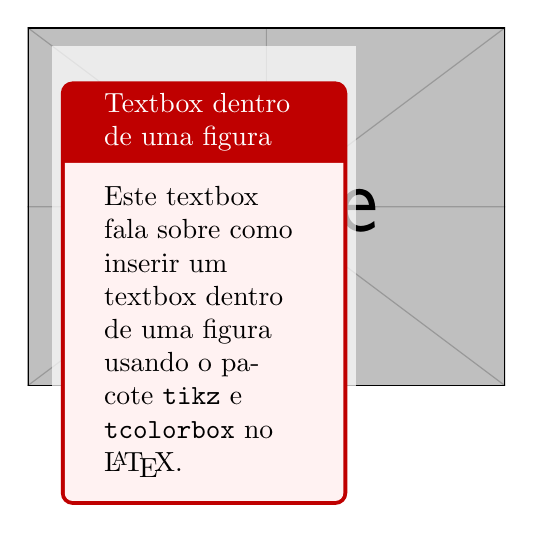
\begin{tikzpicture}
        \node[anchor=south west,inner sep=0] (image) at (0,0) {\includegraphics[width=0.5\textwidth]{example-image}}; % Substitua example-image pelo nome da sua imagem
        \begin{scope}[x={(image.south east)},y={(image.north west)}]
            % Definindo o textbox dentro da figura
            \node[anchor=north west, text width=0.3\textwidth, fill=white, opacity=0.7, text opacity=1] at (0.05,0.95) { % Ajuste a posição conforme necessário
                \begin{tcolorbox}[colback=red!5!white,colframe=red!75!black,title=Textbox dentro de uma figura]
                    Este textbox fala sobre como inserir um textbox dentro de uma figura usando o pacote \texttt{tikz} e \texttt{tcolorbox} no \LaTeX.
                \end{tcolorbox}
            };
        \end{scope}
    \end{tikzpicture}
    \caption{Figura com Textbox}
    \label{fig:figura_com_textbox1}
\end{figure}

\begin{figure}[ht]
    \centering
 \begin{tcolorbox}
Este é o conteúdo do meu textbox sem título. Você pode adicionar qualquer texto aqui, bem como incluir fórmulas matemáticas, listas e outros elementos que desejar. A caixa ajustará automaticamente o tamanho para acomodar seu conteúdo. O textbox agora foi posto dentro de uma figura.
\end{tcolorbox}
    \caption{Figura com Textbox simples}
    \label{fig:figura_com_textbox}
\end{figure}

  \chapter{Método Proposto}
  \chapter{Resultados e Discuss\~oes}

  \section{Algumas Demonstra{\c c}\~oes}

  A  Lista de Símbolos precisa usar comandos específicos. Aqui vamos usar os símbolos $\alpha$ e $\beta$.
  \symbl[beta]{Beta}{A palavra Beta more e corrigida}
  \symbl[zzbeta]{$\beta$}{A letra $\beta$ corrigida}
  \symbl{beta}{A palavra beta}
  \symbl{alpha}{A palavra alpha}
  \symbl[alpha]{Alpha}{A palavra Alpha}
  \symbl[zzalpha]{$\alpha$}{A letra $\alpha$ corrigida}
  \symbl[marco]{Marco}{A palavra Marco corrigida}

  A Lista de Abreviações segue, a partir de 2024, a mesma regra, e aqui seguem alguns exemplos.
  \abbrev{GoT}{Game of Thrones}
  \abbrev[GOT]{GoT}{Game of Thrones ordenado como GOT}
  \abbrev[iot]{IoT}{IoT ordenado como iot}
  \abbrev[IoT]{IoT}{IoT ordenado como IoT}
  \abbrev[IOT]{IoT}{IoT ordenado como IOT}
  \abbrev{IoT}{IoT com ordenação default}
  \abbrev[ITU]{ITU}{ITU mesmo}

  \chapter{Conclus\~oes}

  \backmatter
  \bibliographystyle{coppe-unsrt}
  \bibliography{example}

\appendix

\chapter{Um apêndice}

Segundo a norma da ABNT (Associação Brasileira de Normas Técnicas), a definição e utilização de apêndices e anexos seguem critérios específicos para a organização de documentos acadêmicos e técnicos.

Apêndice: O apêndice é um texto ou documento elaborado pelo autor do trabalho com o objetivo de complementar sua argumentação, sem que seja essencial para a compreensão do conteúdo principal do documento. O uso de apêndices é indicado para incluir dados detalhados como questionários, modelos de formulários utilizados na pesquisa, descrições extensas de métodos ou técnicas, entre outros. Os apêndices são identificados por letras maiúsculas consecutivas, travessão e pelos respectivos títulos. A inclusão de apêndices visa a fornecer informações adicionais que possam ajudar na compreensão do estudo, mas cuja presença no texto principal poderia distrair ou desviar a atenção do leitor dos argumentos principais.

\renewcommand{\appendixname}{Anexo}
\appendix

\chapter{Um Anexo}
Segundo a norma da ABNT (Associação Brasileira de Normas Técnicas), a definição e utilização de apêndices e anexos seguem critérios específicos para a organização de documentos acadêmicos e técnicos.

Anexo: O anexo, por sua vez, consiste em um texto ou documento não elaborado pelo autor, que serve de fundamentação, comprovação e ilustração. O uso de anexos é apropriado para materiais como cópias de artigos, legislação, documentos históricos, fotografias, mapas, entre outros, que tenham relevância para o entendimento do trabalho do autor. Assim como os apêndices, os anexos são identificados por letras maiúsculas consecutivas, travessão e pelos respectivos títulos. Eles são utilizados para enriquecer o trabalho com informações de suporte, garantindo que o leitor tenha acesso a documentos complementares importantes para a validação dos argumentos apresentados no texto principal.
\end{document}

%% 
%%
%% End of file `example.tex'.
